% Provenance (never printed): cycle 4 SVT, "La planete Terre, l'environnement
% et l'action humaine": climate, its past variations and the present change,
% read from data; see sources/book1/PROVENANCE.md. Book 1, grade 9, chapter 1.
% Vocabulary guard: owns climate change (first look; Book 2 g12 re-uses it),
% global warming, temperature anomaly. The greenhouse effect and greenhouse
% gases belong to the chemistry series (grade 8): recalled in prose, never
% defined. Infrared is physics (g10): named in prose only. "Glacial period"
% and "interglacial" belong to Book 2 g12: here "the ice ages and the warmer
% times between them". Physical science only, in the IPCC's calibrated words;
% no policy.
\chapter{地球气候的过去与现在}\label{ch:g9:climate-past-and-present}

设若地球周围没有空气，而其反射的太阳光比例仍与今日相同，
则其表面的平均温度将稳定在
约 \qty{-19}{\degreeCelsius}：海面冰封，陆地冰封，处处如此。
而地球的实际平均温度约为 \qty{15}{\degreeCelsius}。两者之差
约 \qty{34}{\degreeCelsius}，来自空气中的几种气体。它们含量虽微，
却能阻止部分地球热量逸散到太空。
本章讨论的正是这些气体、地球在过去的\omterm{def:g5:weather-and-climate:climate}{气候}，
以及\omterm{def:g5:weather-and-climate:climate}{气候}现今如何、为何正在发生变化。
% ledger: earth:Tbb, earth:Tsurf (figdata/grade-9/climate_records.py: -19.1 and 14.9 degC, gap 34)

\begin{recall}
某地的\omterm{def:g5:weather-and-climate:climate}{气候}，是该地通常\omterm{def:g1:watching-the-weather:weather}{天气}按 30 年平均所得的结果，
（见\cref{ch:g5:weather-and-climate}）。大气最底层，即\omterm{def:g1:watching-the-weather:weather}{天气}发生之处，
是\omterm{def:g8:the-atmosphere:layers}{对流层}。
（见\cref{ch:g8:the-atmosphere}）。\omterm{def:g8:ice-on-earth:ice-age}{冰期}曾多次出现又消退，\omterm{def:g8:ice-on-earth:ice-sheet}{冰盖}远达两极之外，
\omterm{def:g3:continents-and-oceans:poles}{北极}\omterm{def:g8:ice-on-earth:sea-ice}{海冰}自 1979 年以来已经缩小；
（见\cref{ch:g8:ice-on-earth}）。化学课上你已学过，二氧化碳、
甲烷和水汽是\emph{温室气体}：它们使太阳光穿过，
却吸收温暖地面放出的不可见红外线，
这一现象即\emph{温室效应}；燃烧煤、石油
和天然气会释放二氧化碳。
\end{recall}

\section{温室效应与地球的温度}

太阳光穿过大气，加热陆地与\omterm{def:g2:water-on-earth:ocean}{海洋}。与所有温暖的物体一样，
温暖的地表也会以红外线的形式向外辐射能量，
这种红外线为肉眼所不能见。若其全部逸散到太空，地球
就会成为开头所述的冰冻世界。但空气中的温室气体
会吸收大部分红外线，并将其中一部分送回地面：
地表因而既从太阳，又从其上方的空气获得能量，
于是稳定在更高的温度上。

\begin{omfigure}
\begin{tikzpicture}[font=\footnotesize, >={Stealth[length=2.4mm]}]
  % ground and atmosphere
  \fill[omLithAlluv] (0,0) rectangle (12,0.5);
  \fill[omSea!45] (0,0.5) rectangle (12,3.4);
  \node[anchor=north east, align=right] at (11.85,3.35) {大气 \\ 含温室气体};
  \node[anchor=south east] at (11.9,0.05) {陆地与海洋};
  \node[anchor=south west] at (0.15,3.5) {太空};
  % Sun
  \fill[omWxSun] (1.3,5.0) circle (0.45);
  \node at (1.3,4.3) {太阳};
  % sunlight in
  \draw[->, omWxSun!80!black, line width=2.2pt] (1.7,4.6) -- (2.7,0.55)
    node[pos=0.25, right=2pt, align=left, black] {太阳光射入 \\ 并加热地表};
  % infrared out and back
  \draw[->, omWarm, line width=1.6pt, decorate, decoration={snake, amplitude=1mm, segment length=4mm, post length=3mm}]
    (6.0,0.55) -- (6.6,2.6);
  \draw[->, omWarm, line width=1.6pt, decorate, decoration={snake, amplitude=1mm, segment length=4mm, post length=3mm}]
    (6.6,2.7) -- (7.4,5.0) node[right, align=left, black] {部分逸散 \\ 到太空};
  \draw[->, omWarm, line width=1.6pt, decorate, decoration={snake, amplitude=1mm, segment length=4mm, post length=3mm}]
    (6.8,2.75) -- (8.6,0.55);
  \node[align=left, anchor=west] at (8.8,1.9) {部分被气体吸收 \\ 并送回地面};
  \node[align=right, anchor=east] at (5.9,1.3) {温暖的地表 \\ 放出红外线};
\end{tikzpicture}

{\small 温室效应简图（示意）。若无此效应，
地表平均温度约为 \qty{-19}{\degreeCelsius}；有之，
约为 \qty{15}{\degreeCelsius}。}
% ledger: earth:Tbb, earth:Tsurf
\label{fig:g9:climate-past-and-present:greenhouse}
\end{omfigure}

温室效应既是自然现象，也是必需的：没有它，
地表便不会有液态水。本章所关心的是另一个
问题：空气中温室气体的含量
发生变化时，地球的温度会如何变化？

\section{过去的气候}

要读取遥远过去的\omterm{def:g5:weather-and-climate:climate}{气候}，科学家钻探\omterm{def:g8:ice-on-earth:ice-sheet}{冰盖}。
每年都有雪落在\omterm{def:g3:continents-and-oceans:poles}{南极}洲和格陵兰，夏季的雪
与冬季的雪略有不同。雪被掩埋并压实为冰后，
每年形成的层理得以保存，一层压着一层，如同
书页一般。冰越深，年代越久远。
% ledger: eo:ice-core

\begin{omfigure}
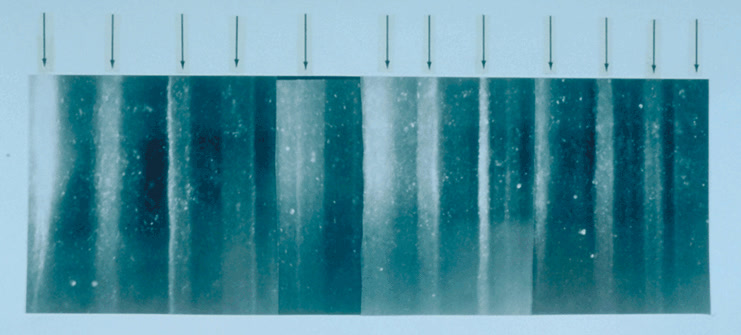
\includegraphics[width=0.78\linewidth]{images/book1/g9-gisp2-layers.jpg}

{\small 一段冰芯，长 \qty{19}{cm}，钻取深度为
\qty{1855}{m} 处，取自格陵兰\omterm{def:g8:ice-on-earth:ice-sheet}{冰盖}，自下方打光。箭头
指向较浅的夏季层，夹在较深的冬季层之间：共
11 年的积雪。NOAA Paleoclimatology（公有领域，经由维基
共享资源）。}
% ledger: commons:gisp2-layers
\label{fig:g9:climate-past-and-present:ice-core}
\end{omfigure}

冰芯保存着两种过去的记录。雪本身能说明
降落时空气的冷暖：空气越冷，雪中
较重的氢、氧同位素所占比例越小。雪被压实时，
颗粒间的空隙闭合，封存了微小气泡，
其中是当时的空气。科学家在
实验室中释放这些古老空气，测量其中的二氧化碳。
% ledger: eo:ice-core

\begin{omfigure}
\begin{tikzpicture}
\begin{axis}[name=temp, omrecord, omage, width=13cm, height=3.9cm, xmin=0, xmax=800,
  xtick={0,100,...,800}, xticklabels={}, ylabel={气温 \\ 变化 ($^\circ$C)},
  ylabel style={align=center}, ymin=-11, ymax=5, ytick={-10,-5,0,5}]
  \addplot[omWarm, line width=0.7pt] table[x=age_kyr, y=temp_C] {figdata/out/grade-9-climate_records-edc.dat};
\end{axis}
\begin{axis}[at={(temp.south west)}, anchor=north west, yshift=-0.3cm, omrecord, omage,
  width=13cm, height=3.9cm, xmin=0, xmax=800, xtick={0,100,...,800},
  xlabel={距今千年前}, ylabel={二氧化碳 \\ (ppm)},
  ylabel style={align=center}, ymin=160, ymax=320, ytick={180,220,260,300}]
  \addplot[black, line width=0.7pt] table[x=age_kyr, y=co2_ppm] {figdata/out/grade-9-climate_records-icecore.dat};
\end{axis}
\end{tikzpicture}

{\small \omterm{def:g3:continents-and-oceans:poles}{南极}冰层记录的八十万年。上图：
Dome~C 处空气温度的变化，与过去
一千年的平均值相比（EPICA Dome~C 冰芯，J.~Jouzel 等，2007）。
下图：冰中封存空气的二氧化碳含量，单位为
百万分之一（B.~Bereiter 等，2015）。两者均以
\num{2000} 年为步长取平均；时间从左（最久远）向右（今天）推进。}
% ledger: data:edc-jouzel, data:co2-bereiter (figdata/grade-9/climate_records.py)
\label{fig:g9:climate-past-and-present:icecore}
\end{omfigure}

两条曲线讲述的是同一个故事。一次又一次，长时间的寒冷期，
即\omterm{def:g8:ice-on-earth:ice-age}{冰期}，让位于较短的温暖期，随后寒冷又会回来。
最冷时，\omterm{def:g3:continents-and-oceans:poles}{南极}上空的气温比过去一千年低约 \qty{9}{\degreeCelsius}；
在最温暖的时期，则只高出几度。
二氧化碳含量与气温同升同降，
在寒冷期约为 \qty{175}{ppm}，在温暖期约为 \qty{300}{ppm}，
我们生活在一个温暖期，
它开始于上一次\omterm{def:g8:ice-on-earth:ice-age}{冰期}结束之时。
% ledger: data:edc-jouzel, data:co2-bereiter (figdata/grade-9/climate_records.py: edc min -9.7, max +3.6; CO2 174 to 299 ppm)

\begin{method}[并排阅读两条记录]
\begin{enumerate}
  \item 检查两条记录是否共用同一时间轴，
        以及时间的推进方向。
  \item 在时间轴上选定一个日期，读取两条记录在该日期的数值。
  \item 寻找峰与谷：两条记录中的峰与谷是否
        在相同时刻出现？
  \item 说明哪些量同步变化，暂不判断哪一个变化
        引起了另一个。
\end{enumerate}
\end{method}

\begin{example}[冰芯中的最后一次冰期]
距今 \num{20000} 年（时间轴上的 20）处，
气温曲线约为 \qty{-9}{\degreeCelsius}，二氧化碳含量约为
\qty{190}{ppm}。过去一千年中，
气温曲线接近 0，二氧化碳含量接近
\qty{280}{ppm}。因此，在末次\omterm{def:g8:ice-on-earth:ice-age}{冰期}最冷时，
\omterm{def:g3:continents-and-oceans:poles}{南极}上空的气温约低 \qty{9}{\degreeCelsius}，
其大气中二氧化碳含量少 $280 - 190 = \qty{90}{ppm}$，约少三分之一。
\end{example}
% ledger: data:edc-jouzel, data:co2-bereiter (figdata/grade-9/climate_records.py: 19-21 kyr bins -9.4, 190 ppm; 1 kyr bin 278)

再往更久远的过去，地球经历过的\omterm{def:g5:weather-and-climate:climate}{气候}远比
最近 800\,000 年中任何时期都要温暖。科学评估认为，
地球表面温度持续高出 19 世纪末水平 \qty{2.5}{\degreeCelsius} 或更多的最后一次，
发生在三百多万年前。
% ledger: ipcc:3myr

\section{当今的记录}

自 19 世纪末以来，每天都在陆地和\omterm{def:g2:water-on-earth:ocean}{海洋}上的
数以千计的\omterm{def:g4:clouds-rain-snow:weather-station}{气象站}测量气温，温度计置于阴凉处。
为了追踪整个星球的温度变化，科学家不直接对气温取平均，
因为各站点的气温本身取决于站点位置；
而是计算每个站点的气温与其自身常年平均值的差值。
% ledger: giss:method

\begin{definition}[温度距平]\label{def:g9:climate-past-and-present:anomaly}
\emph{温度距平}\index{温度距平}是指
某一温度与其在选定参考时段内平均值之间的差。
温度高于该平均值时距平为正，
低于时为负。
\end{definition}

\begin{omfigure}
\begin{minipage}[c]{0.44\linewidth}\centering
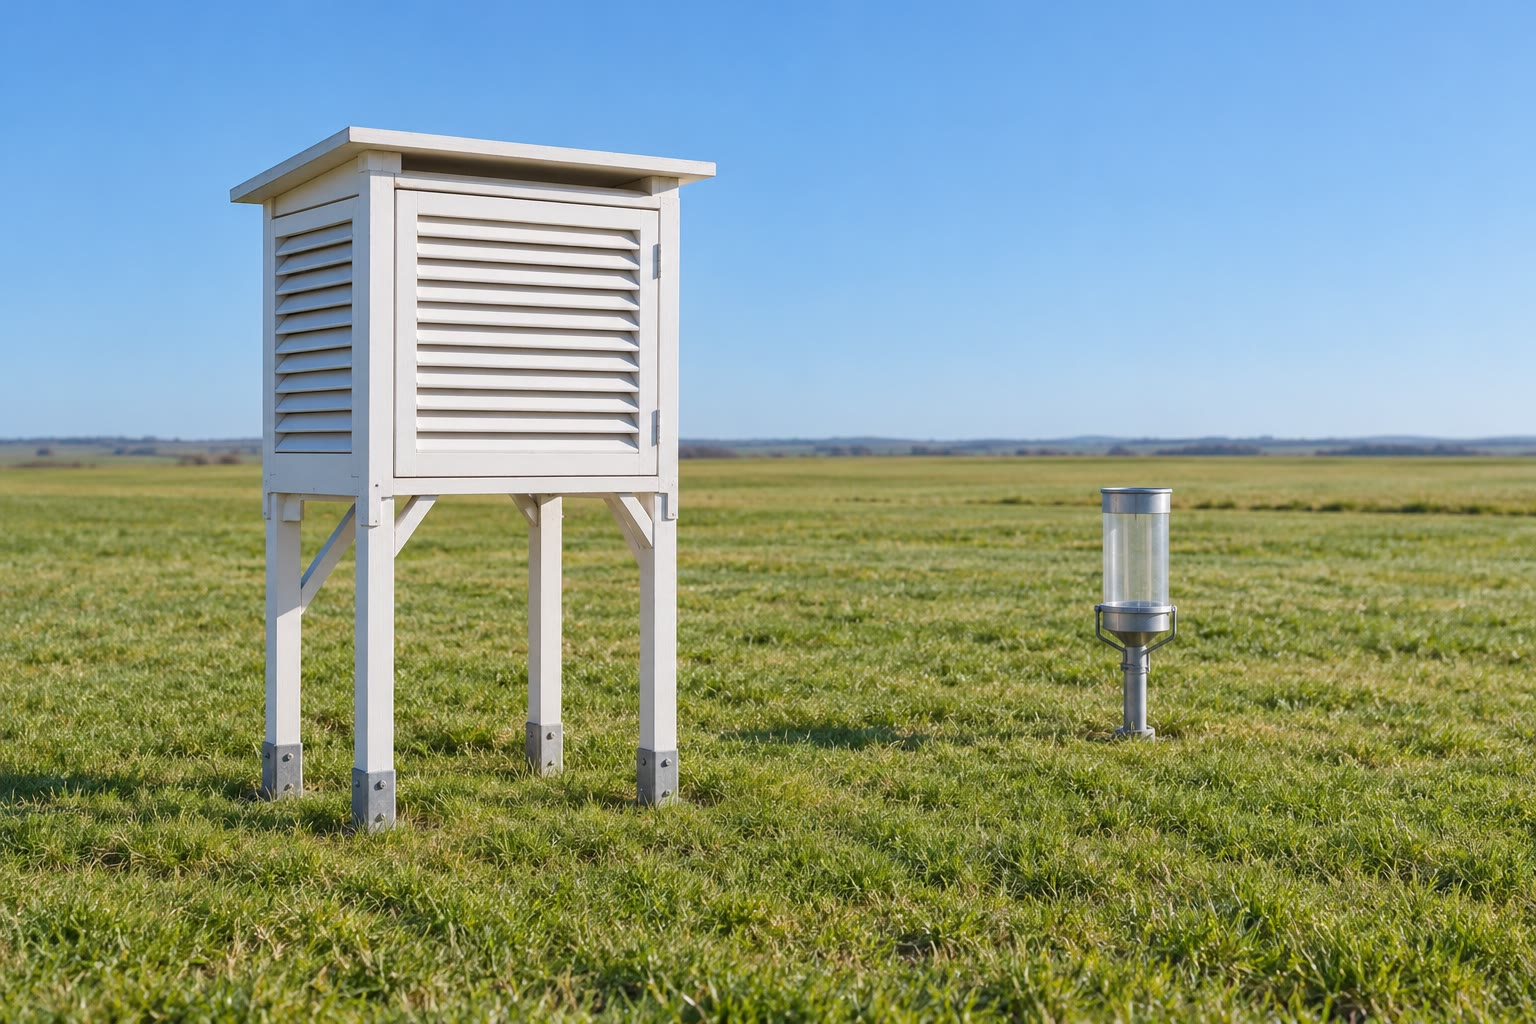
\includegraphics[width=\linewidth]{images/book1/ai/g9-weather-screen.jpg}
\end{minipage}\hfill
\begin{minipage}[c]{0.52\linewidth}\raggedright
{\small \omterm{def:g4:clouds-rain-snow:weather-station}{气象站}：立在支架上的白色箱体，四周为百叶，
使温度计置于阴凉处，空气可从箱体中流过；右侧为\omterm{def:g4:clouds-rain-snow:rain-gauge}{雨量计}
（AI 生成的通用场景示意图）。}
\end{minipage}
\label{fig:g9:climate-past-and-present:screen}
\end{omfigure}

例如，NASA 的全球气温记录给出每年的
\omterm{def:g9:climate-past-and-present:anomaly}{温度距平}，即相对于 1951--1980 年平均值的差，数据来自陆地
\omterm{def:g4:clouds-rain-snow:weather-station}{气象站}与海表温度测量。按十年平均后，
可明显看出气温上升。
% ledger: giss:method, data:gistemp

\begin{omfigure}
\begin{tikzpicture}
\begin{axis}[omrecord, ybar, width=13cm, height=5.6cm, bar width=9pt,
  ymin=-0.45, ymax=1.2, ytick={-0.4,0,0.4,0.8,1.2},
  xtick=data, xticklabels={{1880 年代},{1890 年代},{1900 年代},{1910 年代},{1920 年代},{1930 年代},{1940 年代},{1950 年代},{1960 年代},{1970 年代},{1980 年代},{1990 年代},{2000 年代},{2010 年代},{2020--25}},
  x tick label style={rotate=60, anchor=east, font=\scriptsize},
  ylabel={温度距平 ($^\circ$C)}, xmajorgrids=false]
  \addplot[fill=omWarm!70, draw=black!50] table[x expr=\coordindex, y=mean_C]
    {figdata/out/grade-9-climate_records-decades.dat};
\end{axis}
\end{tikzpicture}

{\small 自 1880 年代起逐十年统计的全球地表温度，
以相对 1951--1980 年平均值的距平表示；最后一根柱覆盖
2020--2025 这六年。数据：NASA GISTEMP version~4。}
% ledger: data:gistemp (figdata/grade-9/climate_records.py)
\label{fig:g9:climate-past-and-present:decades}
\end{omfigure}

\begin{definition}[全球变暖]\label{def:g9:climate-past-and-present:global-warming}
\emph{全球变暖}\index{全球变暖}是指地球表面整体
平均温度自 19 世纪下半叶以来的
上升。
\end{definition}

逐年来看，记录时升时降：某一年可能比前
一年更冷，因为整年的\omterm{def:g1:watching-the-weather:weather}{天气}，无论在\omterm{def:g2:water-on-earth:ocean}{海洋}还是\omterm{def:g3:continents-and-oceans:continent}{大陆}上，
也在波动。要衡量变暖，科学家因此比较
多年的平均值，绝不比较单独两年。

\begin{omfigure}
\begin{tikzpicture}
\begin{axis}[omrecord, width=13cm, height=5.4cm, xmin=1875, xmax=2030, ymin=-0.6, ymax=1.4,
  xtick={1880,1900,...,2020}, x tick label style={/pgf/number format/1000 sep={}},
  xlabel={年}, ylabel={温度距平 ($^\circ$C)},
  legend style={at={(0.2,0.97)}, anchor=north west, draw=none, fill=white, font=\footnotesize}]
  \fill[omWarm!10] (axis cs:1880,-0.6) rectangle (axis cs:1899,1.4);
  \fill[omWarm!10] (axis cs:2015,-0.6) rectangle (axis cs:2024,1.4);
  \addplot[black!70, mark=*, mark size=0.9pt, line width=0.4pt]
    table[x=year, y=anomaly_C] {figdata/out/grade-9-climate_records-annual.dat};
  \addlegendentry{每年}
  \addplot[omWarm, line width=2pt] table[x=year, y=mean_C] {figdata/out/grade-9-climate_records-periods.dat};
  \addlegendentry{时段平均}
  \draw[dashed, black!50] (axis cs:1875,0) -- (axis cs:2030,0);
  \node[font=\scriptsize, fill=white, inner sep=1pt] at (axis cs:1889.5,0.45) {1880--1899};
  \node[font=\scriptsize, fill=white, inner sep=1pt] at (axis cs:2019.5,0.3) {2015--2024};
\end{axis}
\end{tikzpicture}

{\small 1880 至 2025 年每一年的全球\omterm{def:g9:climate-past-and-present:anomaly}{温度距平}
（相对 1951--1980 年平均值，虚线），并给出本章问题中的
两个时段的平均值：1880--1899 与 2015--2024。数据：
NASA GISTEMP version~4。}
% ledger: data:gistemp (figdata/grade-9/climate_records.py)
\label{fig:g9:climate-past-and-present:annual}
\end{omfigure}

\begin{method}[测量两个时段之间的变暖]
\begin{enumerate}
  \item 选取两个时段，每段至少十年，一个较早、
        一个较晚，使单年的起伏相互抵消。
  \item 分别求出每个时段内各年距平的平均值。
  \item 用较晚时段的平均值减去较早时段的平均值，所得结果即
        两个时段之间的变暖量，单位为度。
  \item 说明所用的记录与时段：换用另一套记录，或
        换用其他时段，所得数值会略有不同。
\end{enumerate}
\end{method}

\begin{example}[1970 年代以来的变暖]
在 NASA 记录中，1970--1979 这十年的距平平均为
\qty{0.03}{\degreeCelsius}，而 2010--2019 这十年的平均为
\qty{0.80}{\degreeCelsius}。这两个十年间的变暖量为
$0.80 - 0.03 = \qty{0.77}{\degreeCelsius}$，历时四十年，每十年约
\qty{0.19}{\degreeCelsius}。单个年份即使相隔同样的四十年，
结果也会大相径庭：1976（$-0.10$）与 2016
（1.01）相比得 \qty{1.11}{\degreeCelsius}，而 1979（0.16）与 2011
（0.61）相比只得 \qty{0.45}{\degreeCelsius}。
\end{example}
% ledger: data:gistemp (figdata/grade-9/climate_records.py: decade_1970s 0.03, decade_2010s 0.80; annual 1976 -0.10, 2016 1.01, 1979 0.16, 2011 0.61)

大气中的二氧化碳自 1958 年 3 月起被直接测量，
在夏威夷莫纳罗亚\omterm{def:g4:volcanoes-earthquakes-first-look:volcano}{火山}
山坡约 \qty{3400}{m} 处的一座观测站进行。1959 年，其年平均值为 \qty{316}{ppm}；到
2025 年已达到 \qty{427}{ppm}，远高于它在
800\,000 年冰芯中从未超过的 \qty{300}{ppm}。它的增长越来越快：
1960 年代每年增长不到 \qty{1}{ppm}，最近十年则每年超过
\qty{2.5}{ppm}。
% ledger: gml:keeling, data:co2-mlo, data:co2-bereiter (figdata/grade-9/climate_records.py: 315.98, 427.35, 0.86 and 2.63 ppm/yr; ice core max 298.6)

\begin{omfigure}
\begin{tikzpicture}
\begin{axis}[omrecord, width=12cm, height=5cm, xmin=1955, xmax=2030,
  ymin=290, ymax=440, ytick={300,350,400}, xtick={1960,1970,...,2020},
  x tick label style={/pgf/number format/1000 sep={}},
  xlabel={年}, ylabel={二氧化碳 (ppm)}]
  \addplot[black, line width=0.9pt, mark=*, mark size=0.8pt] table[x=year, y=co2_ppm] {figdata/out/grade-9-climate_records-co2.dat};
  \draw[dashed, omWarm] (axis cs:1955,300) -- (axis cs:2030,300);
\end{axis}
\end{tikzpicture}

{\small 夏威夷莫纳罗亚大气中二氧化碳的年平均值，
1959--2025 年（NOAA 全球监测实验室与斯克里普斯\omterm{def:g2:water-on-earth:ocean}{海洋}
研究所）。虚线处 \qty{300}{ppm} 约为
800\,000 年\omterm{def:g3:continents-and-oceans:poles}{南极}冰芯中发现的最高水平。}
% ledger: data:co2-mlo, data:co2-bereiter (figdata/grade-9/climate_records.py)
\label{fig:g9:climate-past-and-present:co2}
\end{omfigure}

\begin{dated}{2025}
2025 年，莫纳罗亚的二氧化碳年平均值为 \qty{427.35}{ppm}。
在 NASA 记录中，自 1880 年以来最暖的年份是 2024 年，
其距平相对 1951--1980 年为 \qty{1.28}{\degreeCelsius}。
% ledger: data:co2-mlo, data:gistemp (figdata/grade-9/climate_records.py)
\end{dated}

\omterm{def:g4:world-physical-map:altitude}{海平面}也在上升。自 1993 年起，卫星便测量了
全球各处的海面高度：其记录的趋势线
每年约上升 \qty{3.2}{mm}，三十年约上升 \qty{10}{cm}。
\omterm{def:g4:world-physical-map:altitude}{海平面}上升有两个原因：水受热膨胀，以及陆地冰
融化，向\omterm{def:g2:water-on-earth:ocean}{海洋}补充水。冰也在缩小：几乎所有地区的山地\omterm{def:g8:ice-on-earth:glacier}{冰川}
都在后退，\omterm{def:g3:continents-and-oceans:poles}{北极}夏季\omterm{def:g8:ice-on-earth:sea-ice}{海冰}的范围自 1979 年以来已减少
近一半（见\cref{ch:g8:ice-on-earth}）。
% ledger: data:gmsl-lsa (figdata/grade-9/climate_records.py: 3.18 mm/yr; 101 mm 1993-2024), ipcc:b1-ice, nsidc:ice-shelves, data:b1-nsidc-sea-ice

\begin{omfigure}
\begin{tikzpicture}
\begin{axis}[omrecord, width=12cm, height=4.8cm, xmin=1992, xmax=2026,
  ymin=-30, ymax=100, xtick={1995,2000,...,2025},
  x tick label style={/pgf/number format/1000 sep={}},
  xlabel={年}, ylabel={海平面（mm）},
  legend style={at={(0.02,0.97)}, anchor=north west, draw=none, fill=white, font=\footnotesize}]
  \addplot[omCold, mark=*, mark size=1.1pt, line width=0.6pt] table[x=year, y=gmsl_mm] {figdata/out/grade-9-climate_records-sea.dat};
  \addlegendentry{年均值}
  \addplot[omWarm, dashed, line width=0.9pt] table[x=year, y=gmsl_mm] {figdata/out/grade-9-climate_records-sea-trend.dat};
  \addlegendentry{趋势线}
\end{axis}
\end{tikzpicture}

{\small 卫星测得的全球平均\omterm{def:g4:world-physical-map:altitude}{海平面}，年均值
1993--2024 年，相对于参考平面，以及其趋势线（美国国家\omterm{def:g2:water-on-earth:ocean}{海洋}和大气管理局
卫星测高实验室）。}
% ledger: data:gmsl-lsa (figdata/grade-9/climate_records.py)
\label{fig:g9:climate-past-and-present:sea}
\end{omfigure}

\section{气候变化及其成因}

\begin{definition}[气候变化]\label{def:g9:climate-past-and-present:climate-change}
\emph{气候变化}\index{气候变化}是指地球或某一地区
在数十年或更长时间内发生的变化，即其平均温度、\omterm{def:g4:clouds-rain-snow:precipitation}{降水}、
风或冰的状况发生改变，
而非仅仅某个异常的季节。
\end{definition}

冰芯显示，\omterm{def:g5:weather-and-climate:climate}{气候}一直在变化。新的是
今天变化的速度及其成因。世界各地的科学家
定期评估已发表的有关\omterm{def:g5:weather-and-climate:climate}{气候}的研究，并汇总于
政府间\omterm{def:g9:climate-past-and-present:climate-change}{气候变化}专门委员会（IPCC）的报告中。
这些报告会权衡每一项陈述的可靠程度，措辞十分审慎。

在这些报告中，下列每个词都有固定含义：
即该陈述为真的可能性，以百分之几计。

\begin{center}
{\small
\begin{tabular}{|l|c||l|c|}
\hline
\emph{几乎确定} & 99 至 100 & \emph{可能} & 66 至 100 \\
\emph{极有可能} & 95 至 100 & \emph{大致同等可能} & 33 至 66 \\
\emph{很可能} & 90 至 100 & \emph{不太可能} & 0 至 33 \\
\hline
\end{tabular}}
\end{center}
% ledger: ipcc:likelihood

\noindent 有些陈述不含以上任何一词，而是作为事实给出，
例如“\emph{毋庸置疑}”。阅读有关\omterm{def:g5:weather-and-climate:climate}{气候}的新闻报道时，
请留意其中出现的是哪些词，
以及报道保留了哪些、省略了哪些。
% ledger: ipcc:unequivocal

2021 年发布的评估报告给出以下结论。
\begin{itemize}
  \item \emph{毋庸置疑}的是，人类活动已使
        大气、\omterm{def:g2:water-on-earth:ocean}{海洋}和陆地变暖。
  \item 2011--2020 年全球地表温度约
        比 1850--1900 年高 \qty{1.1}{\degreeCelsius}，近四个十年中
        的每一个十年都比自 1850 年以来
        此前的任何十年更暖。
  \item 自 1850--1900 年至 2010--2019 年，\emph{可能}由人类活动引起的变暖
        幅度为 0.8 至 \qty{1.3}{\degreeCelsius}，最佳估计为 \qty{1.07}{\degreeCelsius}，
        几乎占全部观测到的变暖。自然因素合计
        引起的温度变化
        仅为 $-0.1$ 至 $+\qty{0.1}{\degreeCelsius}$。
  \item 2019 年大气中的二氧化碳浓度高于
        至少二百万年以来的任何时期（\emph{可信度高}）；
        且自 1750 年以来上升了 47~\%。
  \item 人类影响\emph{很可能}是
        1990 年代以来\omterm{def:g8:ice-on-earth:glacier}{冰川}退缩和\omterm{def:g3:continents-and-oceans:poles}{北极}\omterm{def:g8:ice-on-earth:sea-ice}{海冰}缩减的主要原因；
        人类影响同样\emph{很可能}是
        至少自 1971 年以来\omterm{def:g4:world-physical-map:altitude}{海平面}上升的主要原因。
\end{itemize}
% ledger: ipcc:unequivocal, ipcc:gsat-2011-2020, ipcc:decades, ipcc:attribution, ipcc:co2-2myr, ipcc:b1-ice, ipcc:sea-level-obs

\begin{history}[基林曲线]
1958 年 3 月，斯克里普斯\omterm{def:g2:water-on-earth:ocean}{海洋}研究所的一位年轻化学家，
查尔斯·戴维·基林开始测量
空气中的二氧化碳，地点为莫纳罗亚山，高出海面、远离任何城镇。
他的测量此后一直持续：这是直接在空气中测得的
二氧化碳的最长记录，其绘出的曲线逐年上升，
即以他的名字命名的\emph{基林曲线}。
% ledger: gml:keeling
\end{history}

为何变暖会跟随二氧化碳的变化？燃烧煤、油和天然气
会释放二氧化碳；空气中二氧化碳越多，意味着
更多地表发出的红外线被吸收并送回
地面，地表因此变暖。水蒸气、甲烷及其他
温室气体也会加强这一效应。过去与现在的证据一致：
冰芯与今日的记录都显示，地球温度与二氧化碳
同步升降。
% ledger: ipcc:attribution, ipcc:co2-2myr

\section{练习}

\begin{exercise}[$\star$]\label{exo:g9:climate-past-and-present:1}
% ledger: earth:Tbb, earth:Tsurf
(a) 若无温室效应，地表平均温度应为多少？
(b) 有温室效应时，地表平均温度又是多少？(c) 温室效应使地表
升温了多少度？(d) 列举两种
温室气体。
\end{exercise}

\begin{exercise}[$\star$]\label{exo:g9:climate-past-and-present:2}
判断下列各项属于\omterm{def:g1:watching-the-weather:weather}{天气}还是\omterm{def:g5:weather-and-climate:climate}{气候}，并说明理由：(a) 昨天下了一整天的雨。(b) 该地区
夏季炎热干燥。(c) 2010 年代的全球气温比 1980 年代高；
(d) 下周将会很冷。
\end{exercise}

\begin{exercise}[$\star$]\label{exo:g9:climate-past-and-present:3}
% ledger: commons:gisp2-layers
看一看这张冰芯切片的照片。(a) 该切片长多少，
其中包含多少年的积雪？(b) 求一年积层的平均
厚度，单位用厘米。(c) 为什么\omterm{def:g8:ice-on-earth:ice-sheet}{冰盖}最深处的
冰最古老？
\end{exercise}

\begin{exercise}[$\star$]\label{exo:g9:climate-past-and-present:4}
某镇 1991--2020 年间七月平均气温为
\qty{21.0}{\degreeCelsius}。求下列七月平均气温的\omterm{def:g9:climate-past-and-present:anomaly}{温度距平}：
(a) \qty{22.4}{\degreeCelsius}；(b) \qty{20.3}{\degreeCelsius}；
(c) \qty{21.0}{\degreeCelsius}。(d) 负的\omterm{def:g9:climate-past-and-present:anomaly}{温度距平}说明什么？
\end{exercise}

\begin{exercise}[$\star\star$]\label{exo:g9:climate-past-and-present:5}
% ledger: data:gistemp (figdata/grade-9/climate_records.py)
利用各十年的柱状图。(a) 哪些十年比
1951--1980 年的平均值更冷？(b) 读出 1980 年代和 2010 年代的距平。
(c) 这两个十年之间距平增加了多少？(d) 从一个十年到下一个十年，
整个记录中的升温是否平稳？
\end{exercise}

\begin{exercise}[$\star\star$]\label{exo:g9:climate-past-and-present:6}
% ledger: data:co2-mlo (figdata/grade-9/climate_records.py)
在茂纳罗亚，年平均二氧化碳浓度在 1959 年为 \qty{315.98}{ppm}，
1969 年为 \qty{324.62}{ppm}，2015 年为 \qty{401.01}{ppm}，2025 年为 \qty{427.35}{ppm}。(a) 1959 年至 1969 年间，
每年平均增加多少？(b) 2015 年至 2025 年呢？(c) 后一时段的
增长速率是前一时段的多少倍？(d) 1959 年至 2025 年间，
二氧化碳浓度增加了百分之多少？
\end{exercise}

\begin{exercise}[$\star\star$]\label{exo:g9:climate-past-and-present:7}
% ledger: data:edc-jouzel, data:co2-bereiter
利用 800\,000 年的记录。(a) 将 800\,000 年写成
科学记数法。(b) 在我们所处的这段温暖期之前，最近一次
与今天一样温暖的时候大约是多久以前？(c) 当时大气中的
二氧化碳浓度是多少？(d) 温度与二氧化碳的
升降是否同步？
\end{exercise}

\begin{exercise}[$\star\star$]\label{exo:g9:climate-past-and-present:8}
% ledger: data:gmsl-lsa (figdata/grade-9/climate_records.py)
\omterm{def:g4:world-physical-map:altitude}{海平面}每年约上升 \qty{3.2}{mm}。(a) 10 年间上升多少，
用厘米表示？(b) 若保持此速率，2025 年至 2100 年间\omterm{def:g4:world-physical-map:altitude}{海平面}将上升多少？
(c) 写出\omterm{def:g4:world-physical-map:altitude}{海平面}上升的两个原因。(d) \omterm{def:g3:continents-and-oceans:poles}{北极}\omterm{def:g8:ice-on-earth:sea-ice}{海冰}融化
会使\omterm{def:g4:world-physical-map:altitude}{海平面}上升吗？请说明理由。
\end{exercise}

\begin{exercise}[$\star\star$]\label{exo:g9:climate-past-and-present:9}
% ledger: ipcc:likelihood
按照 IPCC 的用语，每种表述为真的可能性至少为
100 次中的几次？(a) “\emph{很可能}\ldots”(b) “
\emph{可能}\ldots”(c) “\emph{几乎确定}\ldots”(d) 某报纸
就一个报告中的论断写道“科学家确信”，
而报告将该论断称为\emph{可能}。这种说法有什么问题？
\end{exercise}

\begin{exercise}[$\star\star$]\label{exo:g9:climate-past-and-present:10}
一位朋友说：“这个冬天是我所在地区十年来最冷的一个冬天，
所以地球并没有变暖。”请利用\emph{\omterm{def:g1:watching-the-weather:weather}{天气}}、
\emph{\omterm{def:g5:weather-and-climate:climate}{气候}}和\emph{全球}这几个词，解释这一论证为什么不成立。
\end{exercise}

\begin{exercise}[$\star\star\star$]\label{exo:g9:climate-past-and-present:11}
% ledger: data:co2-bereiter, data:co2-mlo, ipcc:co2-2myr, ipcc:erf-2xco2
在上一次\omterm{def:g8:ice-on-earth:ice-age}{冰期}最冷的时候，约 $2 \times 10^4$ 年前，
大气中约含 \qty{190}{ppm} 的二氧化碳；工业时代之前，
约为 \qty{280}{ppm}；2025 年约为 \qty{427}{ppm}。
(a) 二氧化碳从\omterm{def:g8:ice-on-earth:ice-age}{冰期}增加到工业时代，
增加了多少，历时多少年？(b) 从工业时代到
2025 年，二氧化碳增加了多少？取 1750 年为工业时代的开始。
(c) 比较这两次增加：从增量大小和每年平均增长速率两方面，
用科学记数法进行比较。(d) IPCC 对今天的二氧化碳
浓度与过去相比有何说法？
\end{exercise}

\begin{exercise}[$\star\star\star$]\label{exo:g9:climate-past-and-present:12}
% ledger: ipcc:attribution, ipcc:observed-2010-2019
IPCC 评估给出，从 1850--1900 年到
2010--2019 年的观测升温约为 \qty{1.06}{\degreeCelsius}，人为原因造成的
升温“\emph{可能}”为 0.8 至 \qty{1.3}{\degreeCelsius}（最佳估计
为 \qty{1.07}{\degreeCelsius}）；自然原因合计为
$-0.1$ 至 $+\qty{0.1}{\degreeCelsius}$。(a) 比较人为原因造成升温的最佳估计
与观测升温。(b) 仅靠自然原因能否
解释观测到的升温？请说明理由。(c) 在这句话中，
\emph{可能}是什么意思？
\end{exercise}

\section{问题：行星的温度计}

\begin{problem}[{周末问题——由 NASA 的气温记录推算地球的变暖，
再与二氧化碳和海平面的数据
相比较}]
\label{pb:g9:climate-past-and-present:1}
% ledger: data:gistemp, data:co2-mlo, data:gmsl-lsa, ipcc:gsat-2011-2020 (figdata/grade-9/climate_records.py)
下表给出 NASA 记录中的全球气温距平
（相对于 1951--1980 年的平均值）在若干年份组中的数值，以及
本章其他记录中的数据。

\begin{center}
{\small
\begin{tabular}{|l|c|}
\hline
1880--1899 年平均距平 & \qty{-0.22}{\degreeCelsius} \\
1951--1980 年平均距平 & \qty{0.00}{\degreeCelsius} \\
2015--2024 年平均距平 & \qty{0.98}{\degreeCelsius} \\
茂纳罗亚的二氧化碳，1959 年 / 2025 年 & \qty{316}{ppm} / \qty{427}{ppm} \\
卫星测得的\omterm{def:g4:world-physical-map:altitude}{海平面}趋势，自 1993 年起 & \qty{3.2}{mm} 每年 \\
\hline
\end{tabular}}
\end{center}

\noindent\textbf{第一部分——各时段的平均值。}\par\nopagebreak
\begin{enumerate}[beginpenalty=10000]
  \item 为什么 1951--1980 年的距平恰好为零？
  \item 1880--1899 年比 1951--1980 年更暖还是更冷？相差多少？
  \item 2015--2024 年比 1951--1980 年更暖还是更冷？相差多少？
  \item 计算 2015--2024 年相对于 1880--1899 年的升温幅度。
\end{enumerate}

\noindent\textbf{第二部分——二氧化碳。}\par\nopagebreak
\begin{enumerate}[resume, beginpenalty=10000]
  \item 1959 年至 2025 年间，二氧化碳浓度上升了多少 ppm？
  \item 这一升幅占 1959 年数值的百分之几？
  \item 冰芯记录显示，二氧化碳浓度在 800\,000 年间
        从未超过约 \qty{300}{ppm}。2025 年的数值
        比它高出多少？
  \item 用两句话解释，空气中二氧化碳增多
        如何使地表变暖。
\end{enumerate}

\noindent\textbf{第三部分——\omterm{def:g2:water-on-earth:ocean}{海洋}。}\par\nopagebreak
\begin{enumerate}[resume, beginpenalty=10000]
  \item 按照表中的速率，从 1993 年到 2025 年，\omterm{def:g4:world-physical-map:altitude}{海平面}上升了多少
        厘米？
  \item 说出导致这一上升的两个原因。
  \item 政府间\omterm{def:g9:climate-past-and-present:climate-change}{气候变化}专门委员会（IPCC）给出，2011--2020 年相对于 1850--1900 年的升温
        约为 \qty{1.09}{\degreeCelsius}。你对第 4 题的答案
        与之大小相同吗？请给出一个原因，说明两者
        为何略有不同。
  \item 写出一位科学记者可以刊发的句子：“自
        19 世纪末以来，地球表面已升温
        约 \ldots”
\end{enumerate}
\end{problem}
